\vspace*{0.3cm} \noindent
\subsubsection{Objetivo}
El objetivo de este filtro es transformar el color de una forma determinada llamada "popart".\newline
Se trata de sumar los 3 colores de cada pixel, y según el resultado de esa suma, ir poniendo colores predeterminados.
Formalizando, según el resultado de la suma:\newline


\[ dst_{(x,y)} < r, g, b > = \left\{ \begin{array}{ll}
        < 0, 0, 255 > & \mbox{si $suma(i,j) <153 $}\\
       < 127, 0, 127 > & \mbox{si $153 \leq suma(i,j) <306 $}\\
        < 255, 0, 255 > & \mbox{si $306 \leq suma(i,j) <459 $}\\
       < 255, 0, 0 > & \mbox{si $459 \leq suma(i,j) <612 $}\\
        < 255, 255, 0 > & \mbox{si no}\\\end{array} \right. \]

\vspace*{0.3cm} \noindent

\subsubsection{Desarrollo Implementacion C}

\begin{center}
\textbf{Sintesis de Desarrollo} 
\end{center}

La implementación en C fue simple. Mediante 2 ciclos anidados recorremos la imagen fuente, uno para filas y otro para columnas. \newline
Dentro de la iteración sumamos los colores de cada pixel de la imagen fuente, y según el resultado, pegamos valores predeterminados en la imagen destino.\newline


\begin{center}
\textbf{Explicación detallada de Implementación}

\end{center}

En esta implementación, inicialmente,se crearon dos punteros de matriz uno correspondiente a src y otro a dst.\newline 
Ademas, un entero llamado $suma$ inicializado en 0. \newline
Luego, realizamos dos ciclos, uno añidado dentro del otro recorriendo de la forma $'(int\ i\_d = 0;\ i\_d < filas;\ i\_d++)'$ y 
$(int\ j\_d = 0;\ j\_d < cols;\ j\_d++)$.\newline
Dentro del segundo ciclo, creamos dos punteros rgb\_t donde uno apuntará a \newline rgb\_t $*p\_d = (rgb\_t*)\  \&dst\_matrix[i\_d][j\_d*3]$, y el otro
a $rgb\_t *p\_s = (rgb\_t*)\ \&src\_matrix[i\_d][j\_d]$.\newline
Al entero $suma$ le guardamos la suma de los correspondientes r, g y b del puntero p\_s $suma = p\_s\rightarrow r + p\_s\rightarrow b + p\_s\rightarrow g$ \newline
Posteriormente, chequeamos el valor correspondiente de suma:\newline Primero si $suma < 153$, en caso verdadero, guardamos en el puntero p\_d la posicion 0 de la matriz colores
$*p\_d = colores[0]$. \newline Segundo, si $(153 <= suma \  \&\& \ suma < 306)$, en caso verdadero, guardamos en el puntero p\_d la posicion 1 de la matriz colores
$*p\_d = colores[1]$.\newline Tercero, si $(306 <= suma \  \&\& \  suma < 459)$, en caso verdadero, guardamos en el puntero p\_d la posicion 2 de la matriz colores
$*p\_d = colores[2]$.\newline Cuarto, si $(459 <= suma \  \&\& \  suma < 612)$, en caso verdadero, guardamos en el puntero p\_d la posicion 3 de la matriz colores
$*p\_d = colores[3]$.\newline Por ultimo, si $(612 <= suma)$, en caso verdadero, guardamos en el puntero p\_d la posicion 4 de la matriz colores
$*p\_d = colores[4]$.\newline
Esta matriz colores mencionada se encuentra definida fuera de la funcion como:\newline \noindent
rgb\_t colores[] =  \{ \{255,   0,   0\},\newline
    \hspace*{2.8cm}  \{127,   0, 127\}\,\newline
    \hspace*{2.8cm}               $\{255,   0, 255\}\,$\newline
     \hspace*{2.8cm}              $\{  0,   0, 255\}\,$\newline
	\hspace*{2.8cm}	     $\{  0, 255, 255\} \}\;$
\vspace*{0.3cm} \noindent\newline
Estos dos ciclos realizaran $j\_d = cols - 1$  por $i\_d = filas -1$ de itereaciones.\newline
Con lo mencionado, obtenemos el filtro popart en c correctamente, con los valores que nos pasan como parámetros.\newline

\vspace*{0.3cm} \noindent
\subsubsection{Desarrollo Implementacion en ASM}
En esta implementacion, inicialmente pusheamos RBP, R12 y R13, nos guardamos en R12 y R13 los respectivos valores de columnas y filas.\newline
Luego, guardamos en EAX un 3, guardamos en R10D, R13D y procedemos a hacer la operacion MUL R10, luego realizamos lo mismo con R12 y así,
obtenemos en R10 el valor completo de la cantidad de pixeles a recorrer.\newline
Guardamos en R11 el valor de RDI donde venia *src y en R13 el valor de RSI donde venia *dst. \newline
Luego, realizamos la seccion donde chequeamos si estamos en el final de la linea o mejor dicho en el padding, comparamos con R10D si es cero \newline
en caso de ser 0 significa que ya recorrimos toda la imagen completa por ende saltamos a la etiqueta fin. \newline
En caso de no ser cero, comparamos r15d con 15, en r15 teníamos guardado la cantidad de pixel que vamos a recorrer en una iteracion.
Como vemos de a 15 pixeles si el valor es menor significa que estamos por tocar el padding y eso lo chequeamos a parte. \newline
Si no es menor, procedemos a recorrer y trabajar con 15 pixeles de la siguiente forma: \newline
Primero, nos guardamos en XMM0 los primeros 15 pixeles haciendo $ movdqu\  XMM0, [RDI]$, luego, el valor de XMM0,
lo guardamos en XMM1 y XMM2, limpiamos XMM7 y con 3 mascaras distintas que lo que hacen es ponernos los 5 pixeles rojos adelante y llenar con 0, 
los 5 pixeles azules y llenar con cero y los 5 pixeles verdes y llenar con ceros. \newline
Realizamos la operacion Pshufb con los tres xmm y las mascaras (un xmm con cada mascara) y luego desempaquetamos de byte a word,
usando el xmm7 que habiamos llenado de 0. \newline
El desempaquetado hace que nos queden los valores en word en los registros XMM10, XMM12, XMM14 respectivamente, y luego
los sumamos con PADDW guardando el valor en XMM10. De esta forma obtenemos en word 
$|b0 + g0 + r0|b1 + g1 + r1|b2 + g2 + r2|b3 + g3 + r3|b4 + g4 + r4|$. \newline
Limpiamos todos los registros que usamos, salvo XMM10 y volvemos a guardar en XMM0 el valor de XMM10 procedemos a las comparaciones.
Primero, vamos a comparar si nuestras sumas son mayores a 611, guardamos en XMM14 el valor 611 con una mascara en DW la cual tiene en todos los pack
el 611. Guardamos en XMM15 el valor XMM0 y comparamos con XMM14.
A partir del resultado en XMM15 realizamos lo siguiente:\newline

$\hspace*{2.3cm}$$movdqu\ XMM13, [MASK\_5] $\newline$ 
$\hspace*{2.8cm}$PADDUSW\ XMM10,\ XMM15 $\newline$
$\hspace*{2.8cm}$movdqu\ XMM11,\ XMM15$\newline$
$\hspace*{2.8cm}$pcmpeqw\ XMM14,\ XMM14$\newline$
$\hspace*{2.8cm}$pxor\ XMM11,\ XMM14$\newline$
$\hspace*{2.8cm}$pand\ XMM0,\ XMM11$\newline$
$\hspace*{2.8cm}$pshufb\ XMM15, [MASK\_DE1WORDA3BYTES]$\newline$
$\hspace*{2.8cm}$pand\ XMM13,\ XMM15$\newline$
$\hspace*{2.8cm}$movdqu\ XMM5,\ XMM13$ \newline

En MASK\_5 tenemos en DW los pack de los resultados que da el caso 5 osea $0|FF|FF$. Luego, en\ XMM10 lo usamos para saturar en 1 los casos que ya 
son chequeados para así no pisarlos con los otros casos. \newline
Lo salvamos y lo invertimos osea de 00 a FF y viceversa y luego hacemos un AND con los pack de\ XMM0 para quedarnos con los valores que no dieron TRUE. \newline
Usamos una mascara para que nos acomode todo de 1word a 3 bytes, hacemos otro AND con los valores TRUE y lo guardamos en\ XMM5. \newline

Despues de chequear este caso pasamos al caso 4: \newline

Primero, vamos a comparar si nuestras sumas son mayores a 458, guardamos en XMM14 el valor 458 con una mascara en DW la cual tiene en todos los pack
el 458. Guardamos en XMM15 el valor XMM0 y comparamos con XMM14.
A partir del resultado en XMM15 realizamos lo siguiente:

$\hspace*{2.3cm}$$movdqu\ XMM13, [MASK\_4] $\newline$
$\hspace*{2.8cm}$PADDUSW\ XMM10,\ XMM15 $\newline$
$\hspace*{2.8cm}$movdqu\ XMM11,\ XMM15$\newline$
$\hspace*{2.8cm}$pcmpeqw\ XMM14,\ XMM14$\newline$
$\hspace*{2.8cm}$pxor\ XMM11,\ XMM14$\newline$
$\hspace*{2.8cm}$pand\ XMM0,\ XMM11$\newline$
$\hspace*{2.8cm}$pshufb\ XMM15, [MASK\_DE1WORDA3BYTES]$\newline$
$\hspace*{2.8cm}$pand\ XMM13,\ XMM15$\newline$
$\hspace*{2.8cm}$movdqu\ XMM4,\ XMM13$ \newline

En MASK\_4 tenemos en DW los pack de los resultados que da el caso 4 osea $0|0|FF$. Luego, en XMM10 lo usamos para saturar en 1 los casos que ya 
son chequeados para así no pisarlos con los otros casos. \newline
Lo salvamos y lo invertimos osea de 00 a FF y viceversa y luego hacemos un AND con los pack de XMM0 para quedarnos con los valores que no dieron TRUE. \newline
Usamos una mascara para que nos acomode todo de 1word a 3 bytes, hacemos otro AND con los valores TRUE y lo guardamos en XMM4. \newline

Despues de chequear este caso pasamos al caso 3: \newline

Primero, vamos a comparar si nuestras sumas son mayores a 305, guardamos en XMM14 el valor 305 con una mascara en DW la cual tiene en todos los pack
el 305. Guardamos en XMM15 el valor XMM0 y comparamos con XMM14.
A partir del resultado en XMM15 realizamos lo siguiente:\newline

$\hspace*{2.3cm}$$movdqu\ XMM13, [MASK\_3] $\newline$
$\hspace*{2.8cm}$PADDUSW\ XMM10,\ XMM15 $\newline$
$\hspace*{2.8cm}$movdqu\ XMM11,\ XMM15$\newline$
$\hspace*{2.8cm}$pcmpeqw\ XMM14,\ XMM14$\newline$
$\hspace*{2.8cm}$pxor\ XMM11,\ XMM14$\newline$
$\hspace*{2.8cm}$pand\ XMM0,\ XMM11$\newline$
$\hspace*{2.8cm}$pshufb\ XMM15, [MASK\_DE1WORDA3BYTES]$\newline$
$\hspace*{2.8cm}$pand\ XMM13,\ XMM15$\newline$
$\hspace*{2.8cm}$movdqu\ XMM3,\ XMM13$ \newline

En MASK\_3 tenemos en DW los pack de los resultados que da el caso 3 osea $FF|0|FF$. Luego, en XMM10 lo usamos para saturar en 1 los casos que ya 
son chequeados para así no pisarlos con los otros casos. \newline
Lo salvamos y lo invertimos osea de 00 a FF y viceversa y luego hacemos un AND con los pack de XMM0 para quedarnos con los valores que no dieron TRUE. \newline
Usamos una mascara para que nos acomode todo de 1word a 3 bytes, hacemos otro AND con los valores TRUE y lo guardamos en XMM3. \newline

Despues de chequear este caso pasamos al caso 2: \newline

Primero, vamos a comparar si nuestras sumas son mayores a 152, guardamos en XMM14 el valor 152 con una mascara en DW la cual tiene en todos los pack
el 152. Guardamos en XMM15 el valor XMM0 y comparamos con XMM14.
A partir del resultado en XMM15 realizamos lo siguiente:

$\hspace*{2.3cm}$$movdqu\ XMM13, [MASK\_2] $\newline$
$\hspace*{2.8cm}$PADDUSW\ XMM10,\ XMM15 $\newline$
$\hspace*{2.8cm}$movdqu\ XMM11,\ XMM15$\newline$
$\hspace*{2.8cm}$pcmpeqw\ XMM14,\ XMM14$\newline$
$\hspace*{2.8cm}$pxor\ XMM11,\ XMM14$\newline$
$\hspace*{2.8cm}$pand\ XMM0,\ XMM11$\newline$
$\hspace*{2.8cm}$pshufb\ XMM15, [MASK\_DE1WORDA3BYTES]$\newline$
$\hspace*{2.8cm}$pand\ XMM13,\ XMM15$\newline$
$\hspace*{2.8cm}$movdqu\ XMM2,\ XMM13$ \newline

En MASK\_2 tenemos en DW los pack de los resultados que da el caso 2 osea $7F|0|7F$. Luego, en XMM10 lo usamos para saturar en 1 los casos que ya 
son chequeados para así no pisarlos con los otros casos. \newline
Lo salvamos y lo invertimos osea de 00 a FF y viceversa y luego hacemos un AND con los pack de XMM0 para quedarnos con los valores que no dieron TRUE. \newline
Usamos una mascara para que nos acomode todo de 1word a 3 bytes, hacemos otro AND con los valores TRUE y lo guardamos en XMM2. \newline

Y por último, el caso 1:\newline

Este caso, es particular, ya que invertimos, y chequeamos si los packs que quedan son menores a 153: \newline

$\hspace*{2.3cm}$$movdqa\ XMM14,[MASK\_153]$\newline$
$\hspace*{2.8cm}$			movdqu\ XMM6,\ XMM10 ; me quedo con\ XMM10 y trabajamos  el de\ XMM6$\newline$
$\hspace*{2.8cm}$			pcmpeqw\ XMM7,\ XMM7 ;\ XMM7 = |1|1|1|1|1|1|1|1|1|1|1|1|1|1|1|1$\newline$
$\hspace*{2.8cm}$			pxor\ XMM6,\ XMM7 ; deja en 1 este caso y 0 los casos ya checkeados$\newline$
$\hspace*{2.8cm}$			pand\ XMM14,\ XMM6 ; en\ XMM14 queda los 153 en los lugares que tengo que comparar$\newline$
$\hspace*{2.8cm}$			movdqu\ XMM15,\ XMM0$\newline$
$\hspace*{2.8cm}$			pcmpgtw\ XMM14,\ XMM15 $$\newline$

			A partir del resultado en XMM14 realizamos lo siguiente:\newline

$\hspace*{2.3cm}$$movdqu\ XMM13, [MASK\_1] $\newline$
$\hspace*{2.8cm}$PADDUSW\ XMM10,\ XMM14 $\newline$
$\hspace*{2.8cm}$movdqu\ XMM11,\ XMM14$\newline$
$\hspace*{2.8cm}$pcmpeqw\ XMM15,\ XMM15$\newline$
$\hspace*{2.8cm}$pxor\ XMM11,\ XMM15$\newline$
$\hspace*{2.8cm}$pand\ XMM0,\ XMM11$\newline$
$\hspace*{2.8cm}$pshufb\ XMM14, [MASK\_DE1WORDA3BYTES]$\newline$
$\hspace*{2.8cm}$pand\ XMM13,\ XMM14$\newline$
$\hspace*{2.8cm}$movdqu\ XMM1,\ XMM13$ \newline

En MASK\_1 tenemos en DW los pack de los resultados que da el caso 1 osea $FF|0|0$. Luego, en XMM10 lo usamos para saturar en 1 los casos que ya 
son chequeados para así no pisarlos con los otros casos. \newline
Lo salvamos y lo invertimos osea de 00 a FF y viceversa y luego hacemos un AND con los pack de XMM0 para quedarnos con los valores que no dieron TRUE. \newline
Usamos una mascara para que nos acomode todo de 1word a 3 bytes, hacemos otro AND con los valores TRUE y lo guardamos en XMM1. \newline

Por finalizado, hacemos or entre los XMM1, 2, 3, 4 y 5, y movemos el valor final de XMM1 a XMM0. \newline Comparamos si estamos 
chequeando el borde haciendo $ cmp\  r15d, 15 jl .terminoBorde $ en caso de no ser menor movemos los packs del XMM0 al puntero
en RDI $movdqu\  [RSI], XMM0$, le restamos a r15d y a r10d, la cantidad de pixeles por ciclo y le sumamos a rdi y rsi la cantidad
de pixeles por ciclo. \newline

En caso de que nuestra comparacion diera que es menor a 15, procedemos a: \newline

$\hspace*{2.3cm}$$movdqu [RSI- pixels\_por\_ciclo + r12],\ XMM0 $\newline$
$\hspace*{2.8cm}$		add r11, r8 $\newline$
$\hspace*{2.8cm}$		add r13, r8 $\newline$
$\hspace*{2.8cm}$		mov RDI, r11 $\newline$
$\hspace*{2.8cm}$		mov r11, rdi  $\newline$
$\hspace*{2.8cm}$		mov RSI, r13 $\newline$
$\hspace*{2.8cm}$		mov r13, rsi $\newline$
$\hspace*{2.8cm}$		sub R10D, r15d $\newline$
$\hspace*{2.8cm}$		mov r15d, r14d$ \newline

Como habiamos enuciado inicialmente, en R11 y R13 nos habiamos guardado RDI y RSI respectivamente y en R8 tenemos por parametro
$src\_row\_size$. De esta forma hacemos que en dst se guarden los ultimos pixeles de la linea y baje a la siguiente sin tocar padding.\newline

Esto, como fue explicado, se recorre, hasta que R10D sea igual a 0.


\vspace*{0.3cm} \noindent
\subsubsection{Experimento 1 - saltos condicionales}

	Se desea conocer que tanto impactan los saltos condicionales
	en el código del ejercicio anterior con \verb|-O1|.\\
	Para poder medir esto, una posibilidad es quitar las comparaciones
	al procesar cada pixel. Por más que la imagen resultante no sea correcta,
	será posible tomar una medida del impacto de los saltos condicionales.
	Analizar como varía la performance. 
	
	Si se le ocurren, mencionar otras posibles formas de medir el impacto de los saltos condicionales.
	
	
  \vspace*{0.3cm} 


 Para poder conocer como impactaban los saltos condicionales en la implementacion realizamos distintas mediciones;
 quitando los saltos con y sin optimizacion obteniendo los siguientes resultados:
 Quitando los saltos sin optimizar obtuvimos que, para imagenes de tamaño pequeño (50x100) con 100 iteraciones, el mencionado codigo insume
 una cantidad de 389596 ciclos por cada llamada. A su vez, con imagenes de tamaño mas grande (200x200) utilizando la misma cantidad de iteraciones,
 el codigo nos insume  una cantidad de 1803084 ciclos por llamada, mientras que con imagenes aun mas grande como por ejemplo 512x512 y 1024x768, demanda
 10745530 y 32020980 por llamada respectivamente.
 \vspace*{0.3cm} 
 Mientras que la implementación sin saltos con optimizacion -O1 cosechamos la siguiente información:
 Para imagenes de tamaño pequeño (50x100) con la misma cantidad de iteraciones insume 167132 ciclos por llamada. 
 Con imagenes de mayor tamaño (200x200), demanda 805378 de ciclos.
 Por ultimo con imagenes de tamaño aun mayor (512x512) y (1024x768), emplea 4719143 y 13811050 de ciclos por llamada correspondientemente.
  \vspace*{0.3cm}
 
  Para una mejor representación se realizo un grafico mostrando a simple vista
  las diferencias entre cada tipo de version de la implementacion implementacion.
 \vspace*{0.3cm} \vspace*{0.3cm}
  \begin{center}
 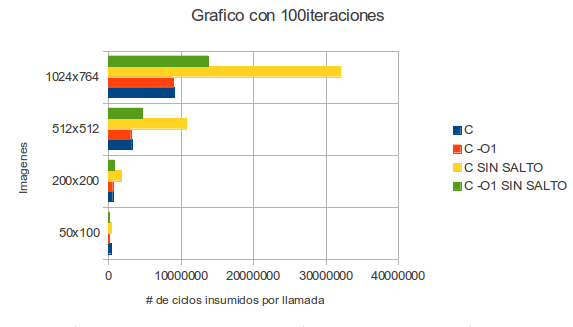
\includegraphics[scale=0.7]{popartbien.png}
 \end{center}
  \vspace*{0.3cm} 

  Concluimos que en imagenes grandes es muy notoria la diferencia en performace entre las versiones con y sin saltos.

\vspace*{0.3cm} \noindent
\subsubsection{Experimento 2 - cpu vs. bus de memoria}

	¿Cuál es el factor que limita la performance en este caso? 
	
	Realizar un experimento, agregando múltiples instrucciones de un mismo tipo
	y realizar un análisis 	del resultado. Acompañar con un gráfico.\vspace*{0.3cm} \noindent

  



  En este caso lo que limita a la performance son las comparaciones y saltos condicionales.
  Para probar esto agregamos instrucciones de varios tipos en la versión de ASM: accesos a memoria, 
  movimiento de registros, sumas, comparaciones y finalmente comparaciones y saltos. \vspace*{0.2cm} \noindent




  Todas estas agregadas en cada instacia de procesamiento, es decir, tomamos el dato, lo procesamos,
  agregamos las instrucciones (50) y así sucesivamente con cada dato.\vspace*{0.2cm} \noindent




  Como resultado observamos que lo que más ciclos insume son las comparaciones y saltos condicionales. 
  Este tipo de instrucciones incrementan con el tamaño de la imagen, ya que mientras mas grande es la imagen, 
  más comparaciones para fijarse si llegó al final tendrá que hacer.\vspace*{0.2cm} \noindent




  Los accesos a memoria también son costosos, pero quedaron en segundo lugar.\vspace*{0.2cm} \noindent
  
  A continuación enunciaremos los respectivos ciclos insumidos por llamada dependiendo cada caso y cada 
  resolución de imagen.\vspace*{0.3cm} \noindent
 
 120x56 
 
+50 accesos		: 124262.398

+50 movimientos		: 85166.438

+50 sumas		: 100156.117

+50 comparaciones	: 106732.922

+50 comp y saltos	: 233104.562

\vspace*{0.3cm} \noindent
200x200

+50 accesos		: 748478.750

+50 movimientos		: 511008.031

+50 sumas		: 584339.938

+50 comparaciones	: 578177.250

+50 comp y saltos	: 1411856.125

\vspace*{0.3cm} \noindent
512x512

+50 accesos		: 5279703.500

+50 movimientos		: 3266983.000

+50 sumas		: 3802452.750

+50 comparaciones	: 4524299.000

+50 comp y saltos	: 9041962.000

\vspace*{0.3cm} \noindent
1023x767

+50 accesos		: 18832506.000

+50 movimientos		: 12843421.000

+50 sumas		: 15499867.000

+50 comparaciones	: 15349734.000

+50 comp y saltos	: 28297848.000

\vspace*{0.3cm} \noindent

  En el siguiente gráfico podemos distinguir los resultados.
  \vspace*{0.2cm} \noindent\vspace*{0.2cm} \noindent


  \begin{center}
 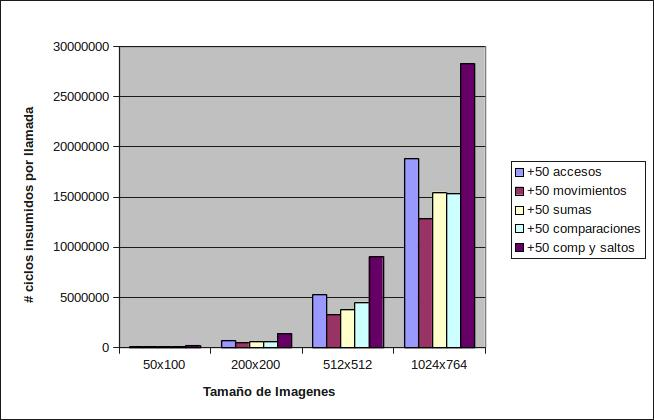
\includegraphics[scale=0.7]{popart2.jpg}
 \end{center}
  \vspace*{0.3cm} 
  


\vspace*{0.3cm} \noindent
\subsubsection{Experimento 3 - prefetch}

  La técnica de \textit{prefetch} es otra forma de optimización que puede
  realizarse. Su sustento teórico es el siguiente:
  
  Suponga un algoritmo que en cada iteración tarda n ciclos en obtener un dato y una cantidad
  similar en procesarlo. Si el algoritmo lee el dato $i$ y luego lo procesa,
  desperdiciará siempre n ciclos esperando entre que el dato llega y que se comienza
  a procesar efectivamente. Un algoritmo más inteligente podría pedir el 
  dato $i+1$ al comienzo del ciclo de proceso del dato $i$ (siempre suponiendo
  que el dato $i$ pidió en la iteración $i-1$. De esta manera, a la vez que el
  procesador computa todas las instrucciones de la iteración $i$, se estáran trayendo
  los datos de la siguiente iteración, y cuando esta última comience, los datos ya
  habrán llegado.  \vspace*{0.2cm}

  

  Estudiar esta técnica y proponer una aplicación al código del filtro en la versión ASM.
  Programarla y analizar el resultado. ¿Vale la pena hacer prefetching?\vspace*{0.2cm}
  
  
  
  
  Cuando empezamos a estudiar esta técnica, creímos que no era realizable en assembler, 
  ya que pensamos que cada instrucción era bloqueante, es decir, 
  que hasta que no se terminaba de ejecutar una instrucción no seguía con la siguiente. \vspace*{0.2cm}
 
 
 
  Luego descubrimos que no era así. El procesador puede ejecutar las instrucciones fuera de orden. 
  Si no es necesario, o no depende de la instrucción anterior, el procesador no espera a que se 
  termine de ejecutar la instrucción actual para ejecutar la siguiente.\vspace*{0.2cm}



  Para probar esto, adaptamos el prefecth a assembler. Modificamos levemente el recorrido de la 
  imagen para no hacer accesos a memoria, al menos no directamente. Lo hicimos a través de un registro.
  Por ejemplo, levantamos de memoria en XMM8, luego lo pasamos a XMM0 y seguimos levantando de memoria 
  la siguiente posición en XMM8. Así mientras se procesa el dato de XMM0 se puede ir trayendo el 
  siguiente dato a procesar en XMM8.\vspace*{0.2cm}
  
  A continuación, enunciaremos los valores obtenidos de nuestras mediciones en las respectivas resoluciones
  utilizando prefecth y sin utilizarlo.\vspace*{0.3cm} \noindent
  
  \vspace*{0.3cm} \noindent
  \vspace*{0.3cm} \noindent
120x56

\vspace*{0.1cm} \noindent

sin prefetch: 67836.359

con prefetch: 65300.320

\vspace*{0.3cm} \noindent
200x200
\vspace*{0.1cm} \noindent

sin prefetch: 398975.594

con prefetch: 382423.562

\vspace*{0.3cm} \noindent
512x512

\vspace*{0.1cm} \noindent

sin prefetch: 2498557.750

con prefetch: 2438276.250

\vspace*{0.3cm} \noindent
1023x767

\vspace*{0.1cm} \noindent

sin prefetch: 10389265.000

con prefetch: 7434984.500

\vspace*{0.3cm} \noindent

 \begin{center}
 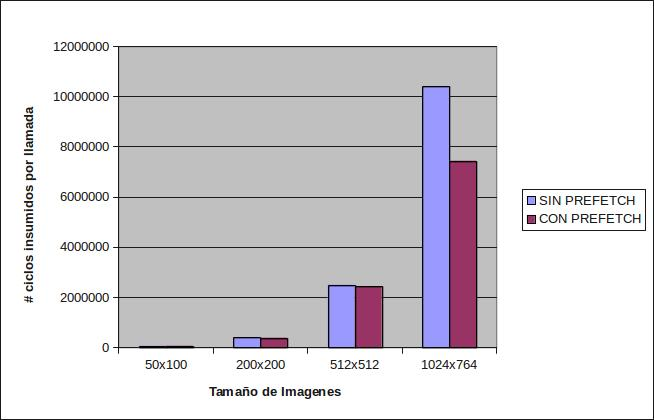
\includegraphics[scale=0.7]{popart3.jpg}
 \end{center}
  \vspace*{0.3cm} 
  
  Se puede observar que hay una sutil mejora en la performance en tamaños pequeños y medianos. 
  En cambio en la imagen grande, se puede observar una brecha más amplia.\vspace*{0.2cm}



  Lógicamente, mientras más grande es la imagen, la mejora será más notoria al haber más accesos a memoria.\vspace*{0.2cm}




  Como conclusión decimos que no vale la pena hacer prefetching para este filtro,
  ya que la diferencia se puede apreciar sólo en imágenes grandes, y además te restringe el uso de un registro XMM.

\vspace*{0.3cm} \noindent
\subsubsection{Experimento 4 - secuencial vs. vectorial}

  Analizar cuales son las diferencias de performace entre las versiones de C y ASM. 
  Realizar gráficos que representen estas diferencias.

  
 Realizando nuestras mediciones en la implementacion de C y en ASM obtenemos los siguientes resultados:\vspace*{0.3cm} \noindent
 
\vspace*{0.3cm} \noindent
120x56

En ASM: 444959

En C: 128763


\vspace*{0.3cm} \noindent
200x200

En ASM: 631827

En C: 628630


\vspace*{0.3cm} \noindent
512x512

En ASM: 3261260

En C: 3098234


\vspace*{0.3cm} \noindent
1023x767

En ASM: 9107332

En C: 8978195


\vspace*{0.3cm}

 Para una mejor representación se realizaron distintos graficos mostrando a simple vista
 las diferencias entre cada tipo de implementacion en cada tipo de imagen.
 \vspace*{0.3cm} \vspace*{0.3cm}
  \begin{center}
 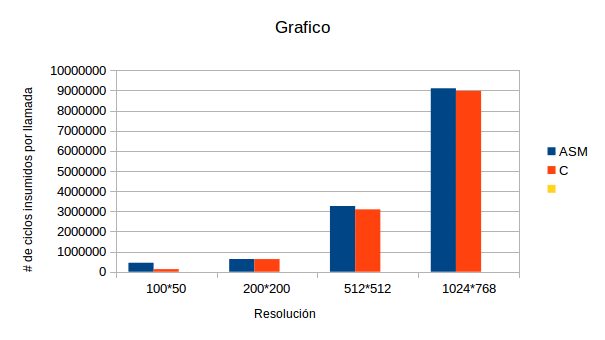
\includegraphics[scale=0.8]{asmc.png}
 \end{center}
  \vspace*{0.3cm} 
  
  La diferencia principal entre el c\'odigo escrito en lenguaje C y el c\'odigo ASM, es la cantidad de accesos 
a memoria realizados en cada iteraci\'on. Otra diferencia puede verse en la cantidad de bytes que pueden 
ser procesados simultaneamente durante el mismo ciclo. 
Mientras que en C leemos y procesamos un byte por vez, el c\'odigo ASM nos permite acceder y procesar 
16 bytes en simultaneos. De todas maneras, en este caso trabajamos con 12 bytes que es un numero mas \'util 
ya que es m\'ultiplo de 3 (cantidad de bytes por p\'ixel)  y de 4 (cantidad de bytes por cada caracter).
Pudiendo levantar de a 16 bytes en memoria, podr\'ia esperarse que el c\'odigo asm demorase una 
diesiseiava parte de la cantidad de ciclos que demora el c\'odigo en C.
Pero debemos tener en cuenta que en nuestro caso estamos aprovechando solo 15 de los 16 bytes que leemos 
en cada iteraci\'on por lo tanto es más acertado evaluar como si solo leyeramos 15 bytes. 
Adem\'as, hay que tener en cuenta que las instrucciones SSE pueden necesitar más ciclos que las operaciones 
comunes que usamos en el C, eso disminuye un poco la performance en la comparación. 
Por mas que como hemos visto los saltos condicionales empeoran la performace en ASM, dicha implementacion
sigue siendo mas optima que la de C.
\vspace*{0.3cm} \vspace*{0.3cm} 
